% !TeX root = ../CCNUthesis.tex

\section{安装}

\subsection{获取 \cls{CCNUthesis}}

目前模块还处于刚开发完的阶段,决定暂时用户以「下载发行版」的方式获取最新版本的 \cls{CCNUthesis}:

\begin{enumerate}
  \item 进入项目主页(\href{https://github.com/xkwxdyy/CCNUthesis}{github 项目主页} (界面见图~\ref{figure:github项目主页} )或 \href{https://gitee.com/xkwxdyy/CCNUthesis}{gitee 项目主页} (界面见图~\ref{figure:gitee项目主页} ))
  \item 在右侧一列有“发行版”(gitee)或“Releases”(github),并且有一个标签图标并有“vx.x.x - 20xx-xx-xx”字样,表示最新的发行版版本和发布时间,点击即可查看相关信息(如果想查看历史所有发行版信息,可以点击“Releases”(github)或“发行版”右侧的“全部”(gitee))。
  
    发行版中一般由以下信息构成(\href{https://github.com/xkwxdyy/CCNUthesis/releases}{github 发行版} 界面见图~\ref{figure:github发行版},\href{https://gitee.com/xkwxdyy/CCNUthesis/releases}{gitee 发行版} 界面见图~\ref{figure:gitee发行版})
      \begin{itemize}
        \item 更新文件的特别说明。如果没有,则表明此次更新只需要更新 \file{CCNUthesis.cls} 文件至最新\footnote{“更新 \meta{文件} 至最新”目前表示在发行版中下载最新版本的模板,并用其中所需要更新的 \meta{文件} 去替换本地的旧 \meta{文件}} 即可
        \item 更新日志。主要为此次发行版与上次发行版的不同,比如“Added”、“Changed”、“Fixed”等等信息
        \item 模版及用户手册下载链接。github 的为“Assets”部分,gitee 的为“下载”部分。一般用户只需要点击 \file{CCNUthesis-vx.x.x.zip} 进行模版下载即可,而下面的 \file{Source code} 为项目的整个源码,包括手册的源码,测试文件等,如果感兴趣的用户可以下载进行查看(当然,如果会使用 \cmd{git} 的用户也可以将整个 \cls{CCNUthesis} 项目 \cmd{clone} 下来查看)
      \end{itemize}
  \item 点击 \file{CCNUthesis-vx.x.x.zip} 进行下载,在本地解压即可
\end{enumerate}

\begin{figure}[htbp]
  \centering
  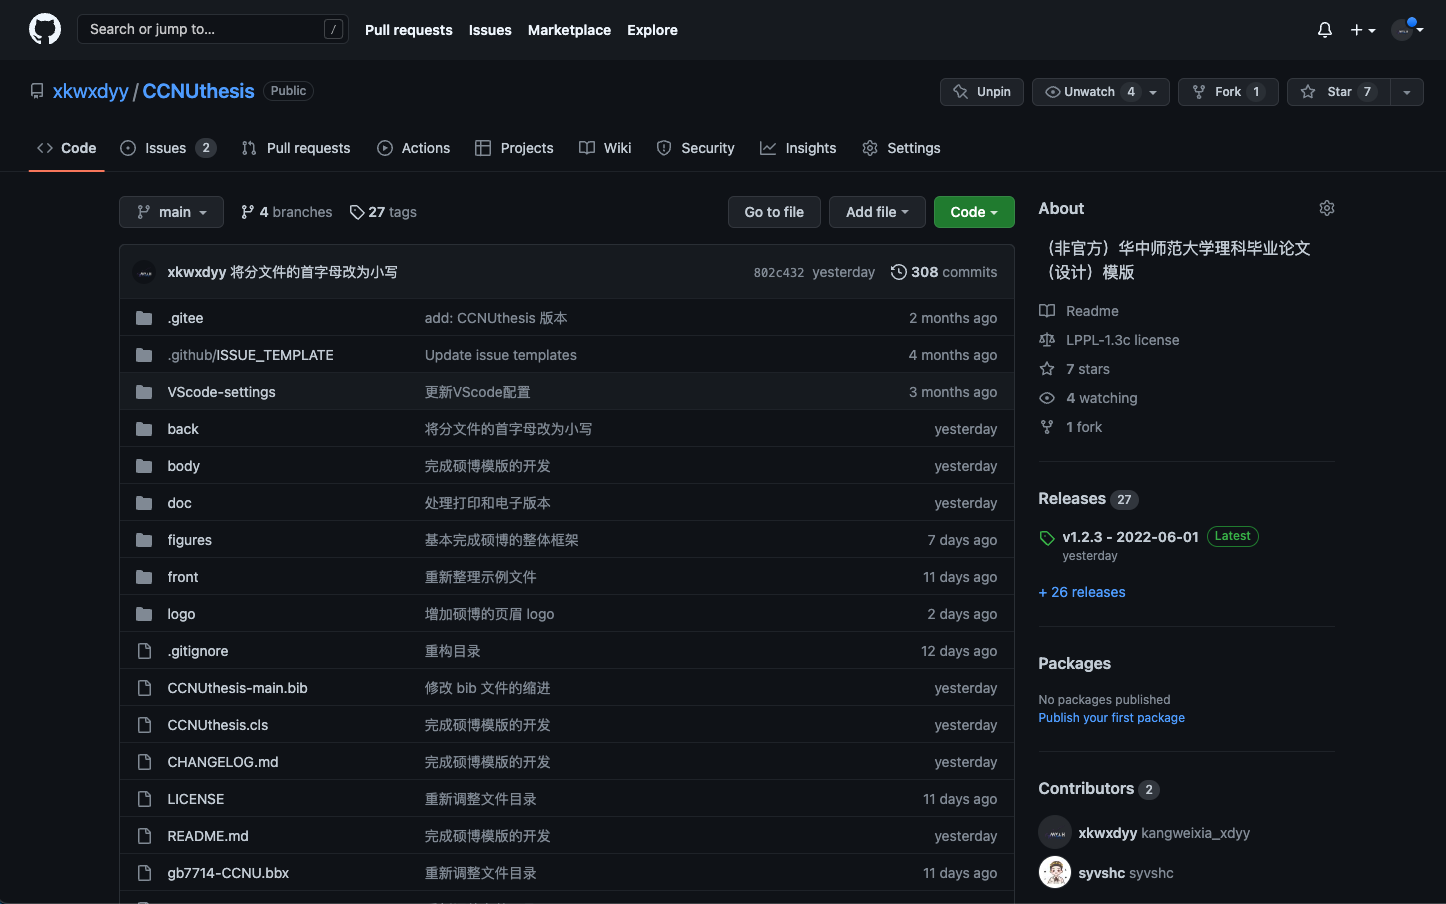
\includegraphics[width = \textwidth]{github项目主页.png}
  \caption{github 项目主页}
  \label{figure:github项目主页}
\end{figure}

\begin{figure}[htbp]
  \centering
  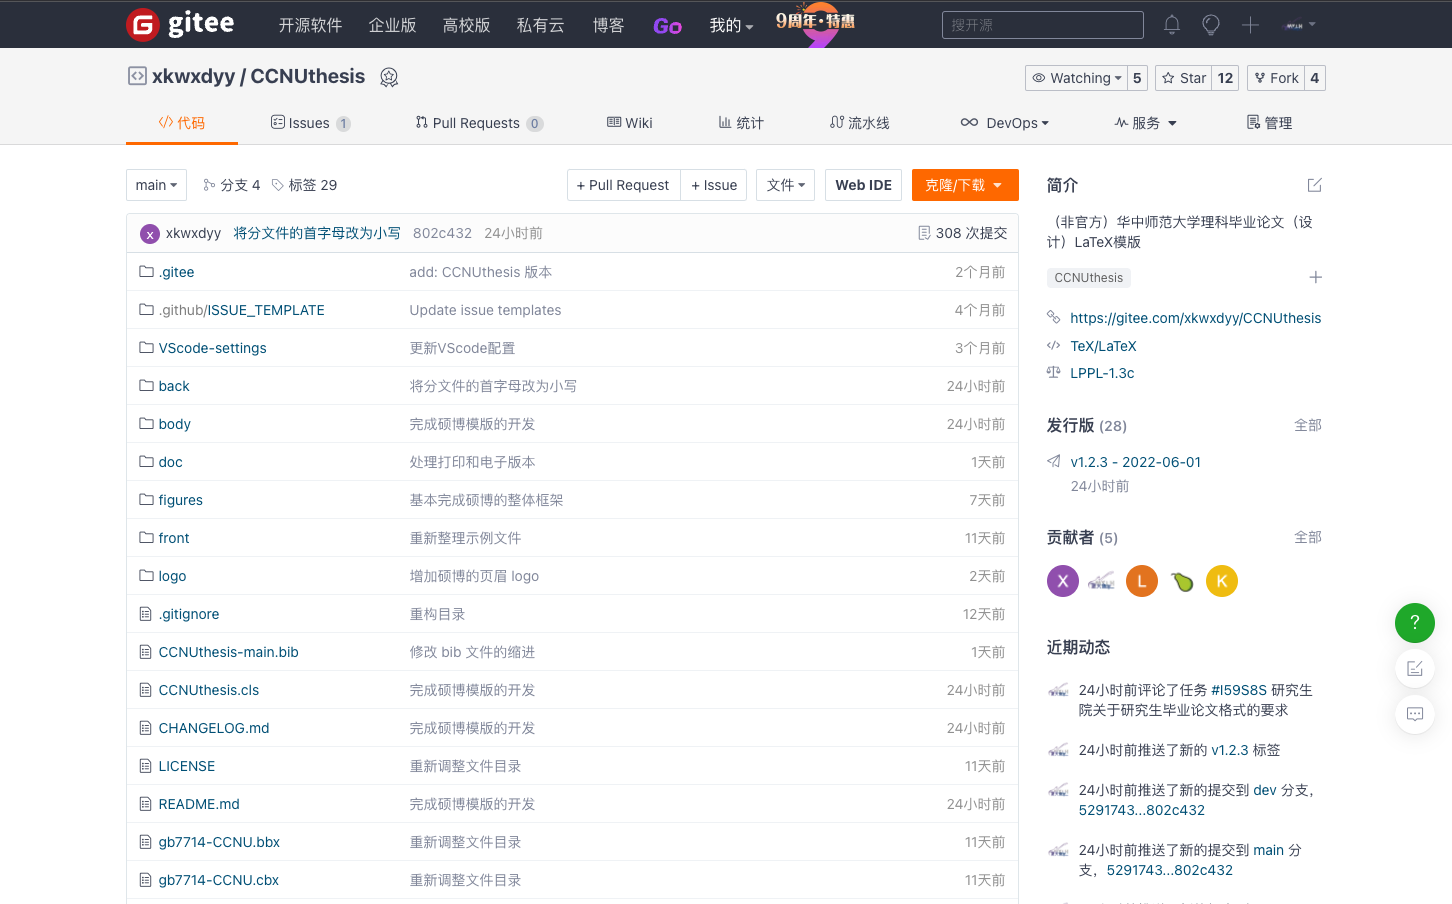
\includegraphics[width = \textwidth]{gitee项目主页.png}
  \caption{gitee 项目主页}
  \label{figure:gitee项目主页}
\end{figure}


\begin{figure}[htbp]
  \centering
  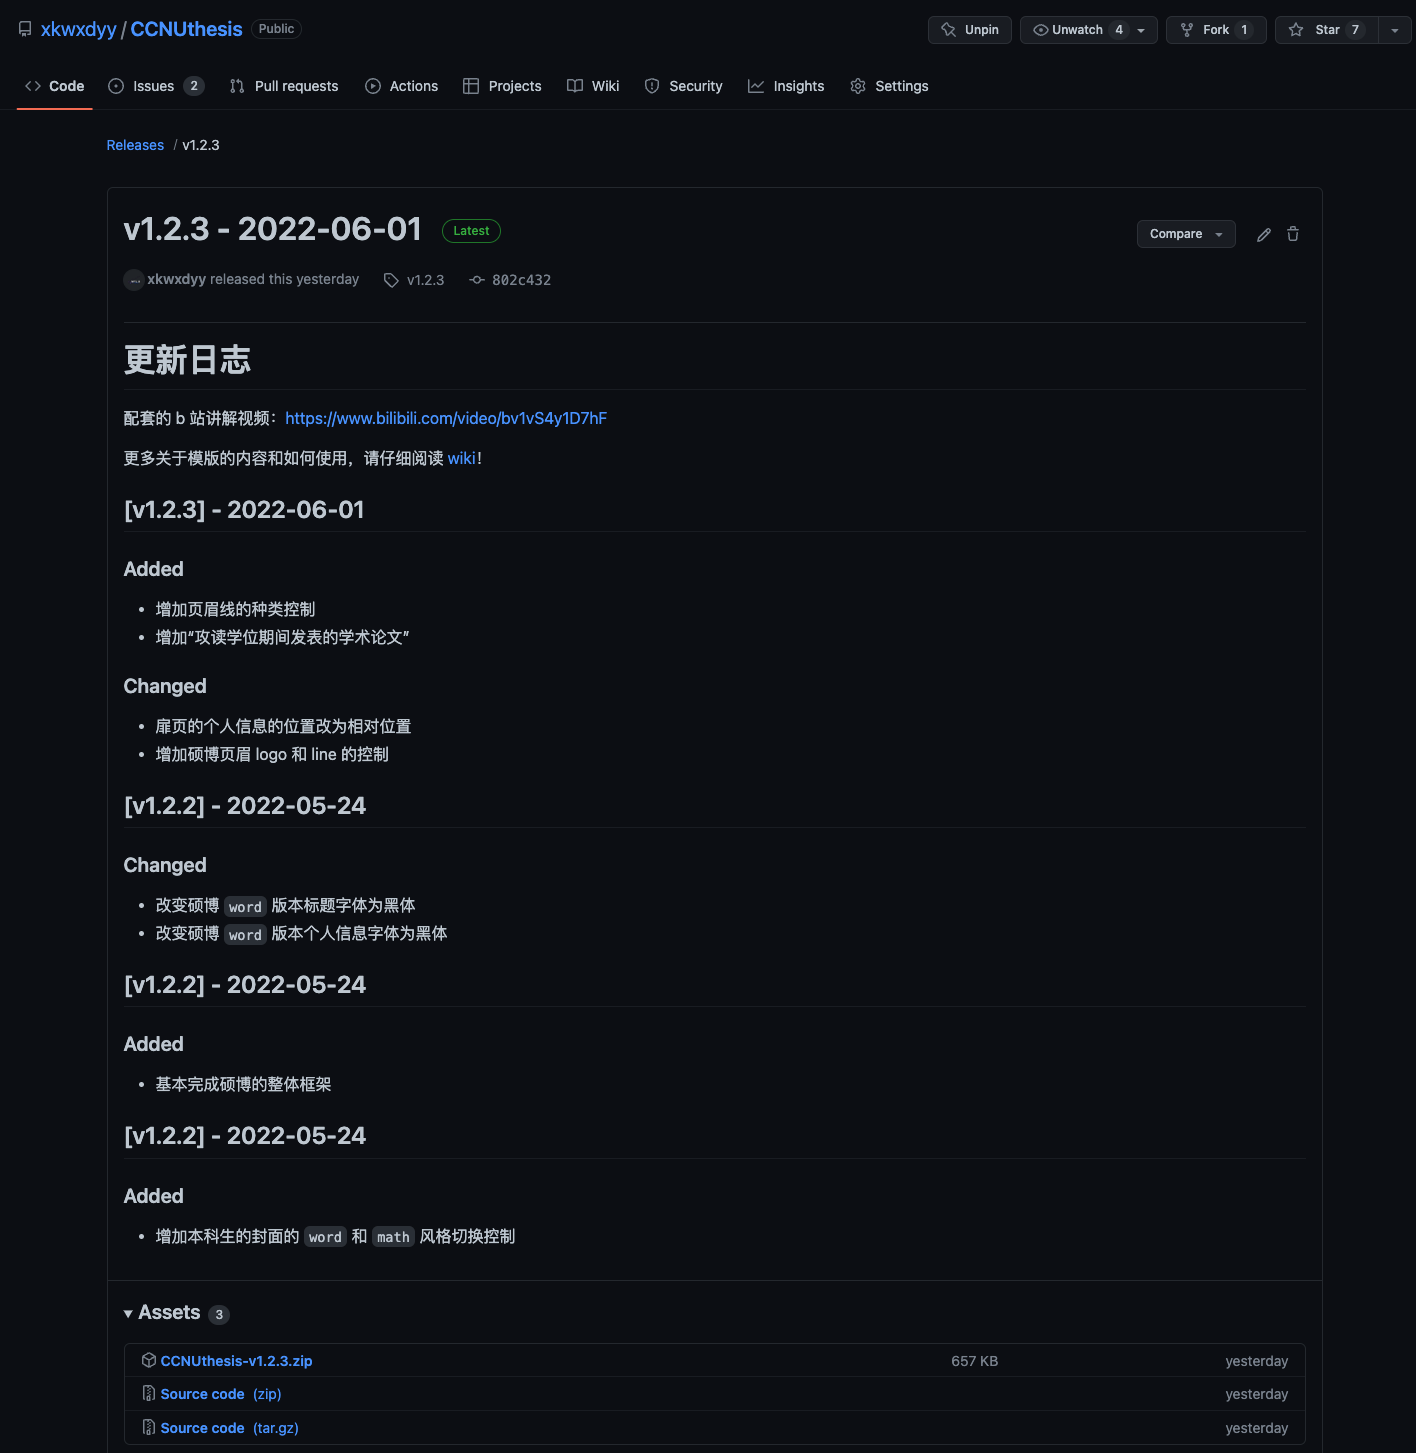
\includegraphics[width = \textwidth]{github发行版.png}
  \caption{github 发行版}
  \label{figure:github发行版}
\end{figure}

\begin{figure}[htbp]
  \centering
  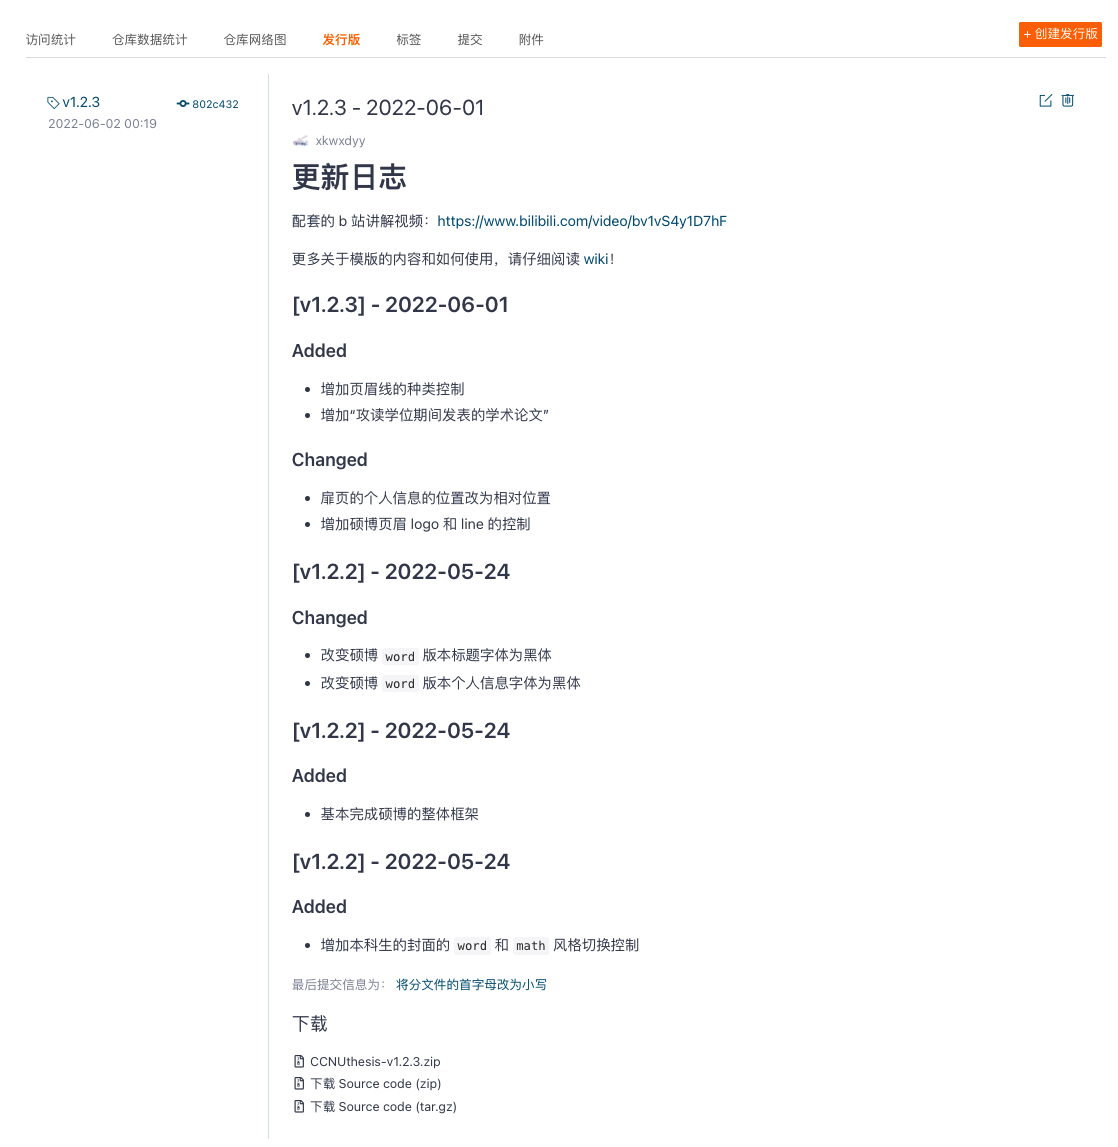
\includegraphics[width = \textwidth]{gitee发行版.png}
  \caption{gitee 发行版}
  \label{figure:gitee发行版}
\end{figure}

% \subsubsection{标准安装}

% 如果没有特殊理由,始终建议您使用宏包管理器安装 \cls{CCNUthesis}。
% 例如在 \TeXLive{} 中,执行(可能需要管理员权限)
% \begin{shellexample}[morekeywords={tlmgr,install}]
%   tlmgr install CCNUthesis
% \end{shellexample}
% 即可完成安装。

% 在 \TeXLive{} 和 \MiKTeX{} 中,您还可以通过图形界面进行安装,
% 此处不再赘述。

% \subsubsection{手动安装}

% 如果您需要从 CTAN 上自行下载并手动安装,较好的方法是使用 TDS
% 安装包:
% \begin{itemize}
%   \item 从 CTAN 上下载 \cls{CCNUthesis} 的
%     \href{http://mirror.ctan.org/install/macros/latex/contrib/CCNUthesis.tds.zip}{TDS 安装包};
%   \item 按目录结构将 \file{CCNUthesis.tds.zip} 中的文件复制到 \TeX{}
%     发行版的本地 TDS 根目录;
%   \item 执行 \bashcmd{mktexlsr} 刷新文件名数据库以完成安装。
% \end{itemize}
% %
% 您也可以从源代码直接生成模板(不推荐):
% \begin{itemize}
%   \item 打开 \href{https://github.com/stone-zeng/CCNUthesis}{项目主页},
%     点击“Code”按钮,并选择“Download ZIP”,下载 \file{CCNUthesis-main.zip};
%     如果您的电脑中安装有 git 程序,也可通过以下命令直接克隆代码仓库:
%     \begin{shellexample}[gobble=6,alsoletter={.},morekeywords={git,clone}]
%       git clone https://github.com/stone-zeng/CCNUthesis.git
%     \end{shellexample}
%   \item 解压并进入到 \file{source} 文件夹,执行以下命令以生成
%     模板的各组件:
%     \begin{shellexample}[gobble=6,morekeywords={xetex}]
%       xetex CCNUthesis.dtx
%     \end{shellexample}
%   \item 将生成的文档类(\file{.cls})、宏包(\file{.sty})以及
%     参数配置文件(\file{.def})复制到 \TeX{} 发行版本地 TDS 树
%     的 \path{texmf-local/tex/latex/CCNUthesis/} 目录下,并执行
%     \bashcmd{mktexlsr} 刷新文件名数据库,方可完成安装。
%   \item 使用 \cls{CCNUthesis} 撰写论文时,您还需要从代码仓库下的
%     \file{testfiles/support} 目录中复制 \file{fudan-name.pdf}
%     文件至工作目录,以确保封面中的校名图片可以正确显示。
% \end{itemize}

% \subsubsection{扁平化安装}

% 如果您不希望安装本模板,但需要立刻使用,也可以使用模板提供的安装脚本。
% 从 GitHub 上获取代码仓库后,执行 \file{install-win.bat}(Windows 系统)
% 或 \file{install-linux.sh}(Linux 系统),所有需要的文件便会在
% \file{thesis} 文件夹中生成。


\subsection{模板组成}

本模板主要包含核心文档类、参考文献格式文件以及用户文档等几个部分,
其具体组成见表~\ref{tab:ccnuthesis-main-components},模版子目录中的文件组成见表~\ref{tab:ccnuthesis-sub-components}。

\begin{table}[htbp]
  \caption{\cls{CCNUthesis} 的主要组成部分}
  \label{tab:ccnuthesis-main-components}
  \centering
  \small
  \begin{tblr}{
    hline{1, 2, Z} = {1pt},
    width = \textwidth,
    colspec = {X[2,l]X[5,l]},
    rows = {m}
  }
    \textbf{文件} & \textbf{功能说明} \\
    \file{CCNUthesis.pdf}         & 用户手册(本文档) \\
    \file{lguide-ch1.pdf}         & \TeXLive 安装指导 \\
    \file{main.tex}               & 模板的主文件,可据此为基础完成论文撰写 \\
    \file{ccnu-setup.tex}         & 用户的个人信息和论文相关参数设置的配置文件\\
    \file{CCNUthesis.cls}         & 模板文档类 \\
    \file{CCNUthesis-main.bib}    & 参考文献数据库文件,里面的条目均为示例,可删除后输入用户自己的参考文献条目并在正文中进行引用 \\
    {\file{gb7714-CCNU.bbx} \\ \file{gb7714-CCNUay.bbx}} & 参考文献的条目格式文件 \\
    \file{gb7714-CCNU.cbx}        & 参考文献的引用格式文件 \\
    \file{latexmkrc}              & \pkg{latexmk} 编译命令的配置文件 \\
    \file{README.md}              & 简要自述 \\
    \file{CHANGELOG.md}           & 模板更新日志 \\
    \file{LICENSE}                & 模版发布许可证
  \end{tblr}
\end{table}

\begin{table}[htbp]
  \caption{\cls{CCNUthesis} 各目录的组成部分}
  \label{tab:ccnuthesis-sub-components}
  \centering
  \small
  \begin{tblr}{
    hline{4,5,8,11,13} = {solid},
    hline{1, 2, Z} = {1pt},
    width = \textwidth,
    colspec = {X[1,l]X[3,l]X[3,l]},
    rows = {m},
    cell{2}{1} = {r=2}{m},
    cell{5}{1} = {r=3}{m},
    cell{8}{1} = {r=3}{m},
    cell{11}{1} = {r=2}{m},
  }
    \textbf{子目录} & \textbf{子目录中的文件} & \textbf{功能说明} \\
    front & \file{abstract.tex}            & 中英文摘要 \\
    front & \file{notation.tex}            & 符号表 \\
    body  & \file{chapter<number>.tex}     & 正文的分文件 \\
    back  & \file{acknowledgements.tex}    & 致谢 \\
    back  & \file{appendix.tex}            & 附录 \\
    back  & \file{publications.tex}        & 攻读学位期间取得的研究成果(博士)\\
    logo  & \file{ccnulogo.png}            & “华中师范大学”字样 logo \\
    logo  & \file{masterlogo.png}          & 硕士学位论文页眉 logo \\
    logo  & \file{doctorlogo.png}          & 博士学位论文页眉 logo \\
    copyright  & \file{Originality_Copyright.pdf}  & 本科学位论文原创性声明和使用授权说明 \\
    copyright  & \file{Originality_Copyright_master_doctor.pdf}  & 硕博学位论文原创性声明和使用授权说明\\
    figures & & 用户放置图片的目录\\
  \end{tblr}
\end{table}